\chapter{Week 05}

    For this week, there was more progress achieved with the turtle simulations, and the process of incorporating Gazebo into JupyterLab was commenced. 

\section{Turtlesim IV}
    
    The turtle widgets were successfully merged into the \texttt{jupyros} repository (\href{https://github.com/RoboStack/jupyter-ros/pull/94}{PR \#94}) after some minor changes which involved creating a separate file for the \texttt{TurtleSim} class. Additionally, thanks to the newest \texttt{ipycanvas} release $0.12.0$, the frame rate of the turtle animations was able to improve by $0.02\ s$ (\href{https://github.com/RoboStack/jupyter-ros/pull/97}{PR \#97}). 


\section{Gazebo II}

    To test if a connection to Gazebo was possible without the GUI, the idea of running a headless Gazebo was explored. However, after several failed attempts it was discovered that the \texttt{"headless"} argument is deprecated (\href{https://github.com/ros-simulation/gazebo_ros_pkgs/issues/491}{\texttt{gazebo\_ros\_pkgs} issue \# 491}) and what was actually needed was simply to set \texttt{"gui"} to False.

    The next test comprised of displaying a robot on GzWeb. With the classic Gazebo application and with the help of the Gazebo ROS packages, a user can simply launch a file which will automatically spawn a robot and any desired world in the Gazebo application. Technically, this should also be possible with the GzWeb client if the communication to the gzserver is properly established. To confirm this, the Gazebo packages for the panda robot and the turtlebot3 were utilized. Initially, GzWeb was unable to display the robots because it could not locate the robots' description packages. As a temporary fix, these description packages were manually copied to the \texttt{assets} directory of GzWeb. Nonetheless, the test failed for the turtlebot3 but it partially passed for the panda robot. The panda robot was able to spawn in GzWeb but it required heavy manipulation of the default launch file to avoid all the errors.
    
    Additionally, it was discovered that GzWeb works better with Chrome than with Firefox. As mentioned last week, the tab buttons on the left panel make the entire panel disappear without sign of return when used with Firefox, however, these buttons are fully functional in Chrome. With a fully functional panel, a turtlebot was finally able to be displayed on GzWeb, but the material textures were still not loading correctly.
    
    For display purposes, additional time was dedicated for building the thumbnails for the models. With the thumbnails, the menu on the left panel for adding new models to GzWeb can display a small preview of each model. Several attempts were required to build the thumbnails, however, once the process was completed a few thumbnails were still not able to be generated.
    
    
    \begin{figure}[ht]
        \centering
        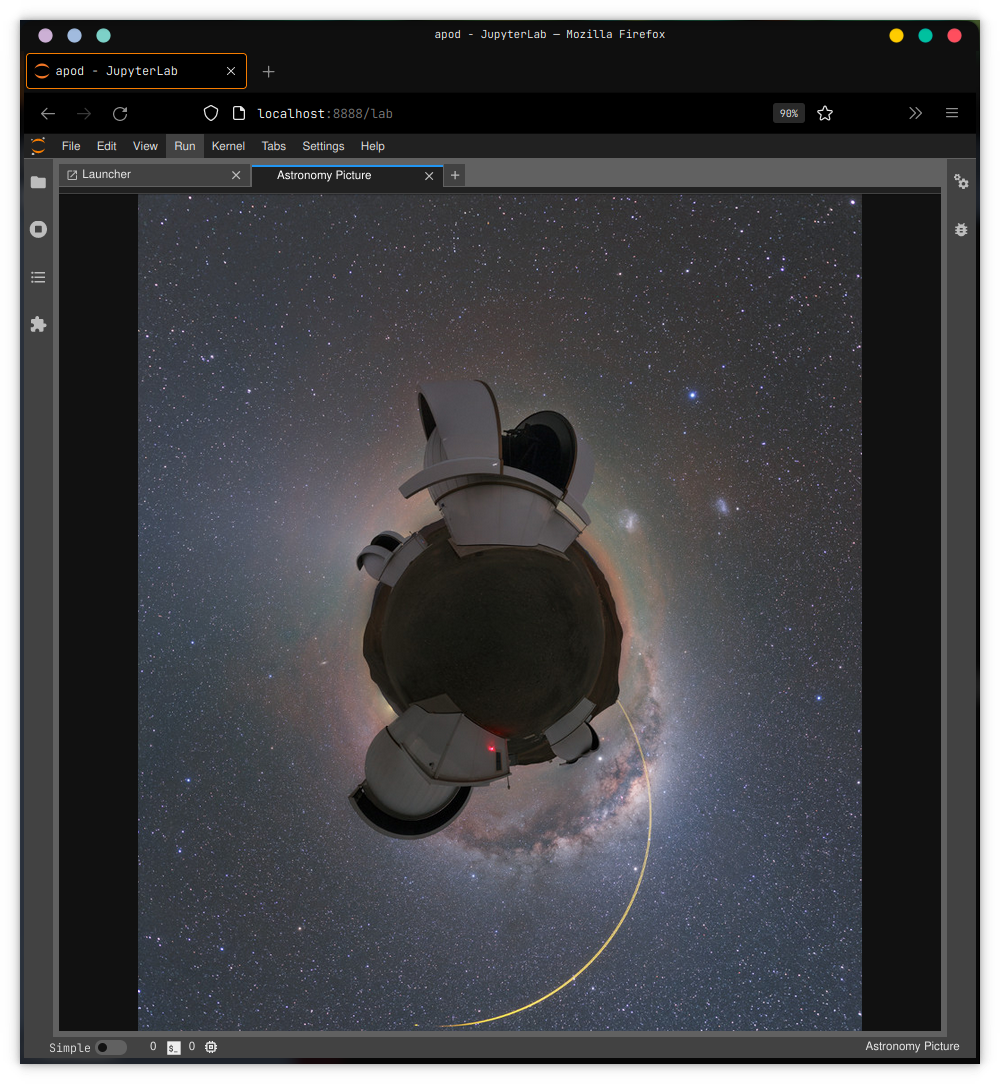
\includegraphics[width=0.7\linewidth]{Images/05_astronomy.png}
        \caption{JupyterLab extension displaying a random astronomy picture.}
        \label{fig:astro}
    \end{figure}

\section{JupyterLab Extensions}
 
    In order to prepare for integrating Gazebo into JupyterLab, I needed to acquire more knowledge in the development of JupyterLab extensions. For this, I followed some of the basic extension examples provided on the JupyterLab documentation.

    \subsection{Astronomy Picture of the Day}
    
    The Astronomy Picture of the Day or \texttt{apod} shown in Figure \ref{fig:astro} is the result of one of the extension examples. With this example I learned to add a command to the command palette, fetch information from the internet, display that information on a new tab panel, and how to style such a panel.
    
    \subsection{TypeScript}
    
    To familiarize myself with TypeScript, I complete all the tutorials from the \href{https://www.w3schools.com/typescript/index.php}{W3Schools}. These covered all the basics of variable types to functions and classes. Although more practice is required to become competent in the language, the tutorials were sufficient to follow through the JupyterLab extension tutorials. 
    
\section{Future Work}

    Although there are several issues with the GzWeb client, the next steps will focus on the development of the Gazebo extension for JupyterLab. Ideally, the issues with GzWeb will be resolved along the way. The solutions will include automating the process for linking the desired media files to GzWeb, this could be accomplished by updating the Python 2 scripts which come with the application. Along the same lines, the generation of thumbnails for the models could also be simplified.
